\documentclass[10pt]{beamer}
\usepackage{tikz}
\tikzstyle{every node}=[circle, draw, fill=black!100, inner sep=0pt, minimum width=5pt]

\usepackage{amsthm}
\usepackage{amssymb}
\usepackage{amsmath}
\usepackage{graphicx}

\usepackage{mathrsfs}

\usepackage{lmodern}

%\usepackage[hang,scriptsize]{subfigure}

\usepackage[format=hang,font={scriptsize}]{caption}
\usepackage[format=hang,font={scriptsize}]{subcaption}

\usepackage{animate}
\usepackage{movie15}

%\usepackage{epsfig}
%\usepackage{tikz-3dplot}

%\usepackage{beamerthemesplit}

\usetheme{CambridgeUS}
\usecolortheme{beaver}

%\setbeamertemplate{footline}{}
%\setbeamertemplate{navigation symbols}{}
%\setbeamercovered{dynamic}
%\hypersetup{pdfpagemode=FullScreen}


\title[Statistical Mechanics Presentation]{Superconductors}
\author[W. Bowman]{\Large Wesley A. Bowman}
\institute[Acadia University]{\Large Acadia University \\ \normalsize Physics Department}
%\titlegraphic{\includegraphics[width=20mm]{Acadia_logo}}


%\hypersetup{pdfpagemode=FullScreen}
%\setbeamertemplate{footline}[page number]{}
\setbeamertemplate{navigation symbols}{}
\setbeamertemplate{caption}[numbered]

\newtheorem{defn}{Definition}
\newtheorem{lem}{Lemma}
\newtheorem{thm}[lem]{Theorem}
\newtheorem{cor}[lem]{Corollary}

\theoremstyle{definition}
\newtheorem{ex}{Example}


\begin{document}

\begin{frame}
    \titlepage
\end{frame}

%%%%%%%%%%%%%%%%%%%%%%%%%%%%%%%%%%%%%%%%%%%%%%%%%%%%%%%%%%%%%%%%%%%%%%%%%%%%%%

\section{Introduction}

\begin{frame}
    \frametitle{Type I or Type II}

    There are two types of superconductors, Type I and Type II\@.
    \\~\\

    When the magnetic field becomes too strong, the system becomes 
    a metal again. Type I superconductors demonstrate this type of behaviour.
    \\~\\

    Type II superconductors act a bit differently.
    Under a small magnetic field, they react like type I superconductors
    and completely expel the magnetic field. But when the magnetic field 
    is stronger, they prefer to adopt a compromise situation and allow 
    some of the magnetic field to penetrate along vortices. Each vortex is a
    small region in a superconductoring metal that acts like a normal metal.
    \\~\\

    The material then becomes a sieve. In order to enable this magnetic 
    field to go through the vortex, the material develops superconducting 
    currents circulating around this pillar in a spiral motion justifying 
    the name vortex.

\end{frame}


\begin{frame}
    \frametitle{Type I or Type II}

    \begin{center}
    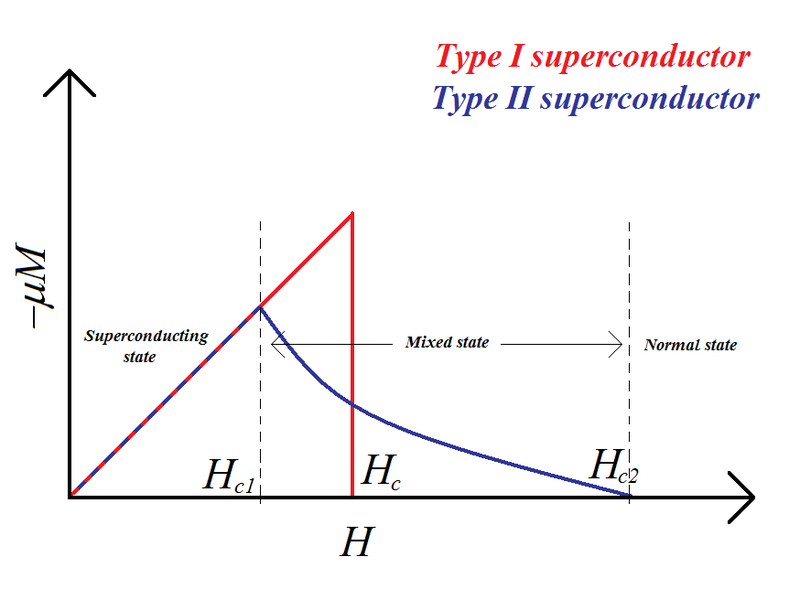
\includegraphics[scale = 0.3]{Magnetisation_and_superconductors}
    \end{center}

\end{frame}


\begin{frame}
    \frametitle{Coherence Length and London Penetration Depth}

    Coherence length is defined as
    \begin{equation}
        \xi = \frac{2 \hbar v_F}{\pi \Delta}
    \end{equation}
    where $v_F$ is the Fermi velocity, and $\Delta$ is the superconducting
    energy gap.
    \\~\\

    The London penetration depth is defined as
    \begin{equation}
        \lambda = \sqrt{\frac{mc^2}{4\pi n_s e^2}}
    \end{equation}
    where $m$ is the mass of the electon, $e$ is the charge of an electon, and
    $n_s$ is the number density of superconducting carriers.

\end{frame}

\begin{frame}[<+->]
    \frametitle{Ratio of the Two}

    Now, the penetration depth and the coherence length both diverge as the
    critical temperature, $T_C$.
    \begin{equation}
        \lim_{T\rightarrow T_C} \xi(T) = \frac{\xi(0)}{\sqrt{1-(T/T_C)}} \qquad
        \lim_{T\rightarrow T_C} \lambda(T) = \frac{\lambda(0)}{\sqrt{1-(T/T_C)}}
    \end{equation}
    But, if we take a ratio of the two, it will be independent of temperature.

    \begin{equation}
        \kappa \equiv \frac{\lambda}{\xi}
    \end{equation}

    For a Type I superconductors,
    \begin{equation}
       0 < \kappa < 1/\sqrt{2}
    \end{equation}

    For Type II superconductors,
    \begin{equation}
        \kappa > 1/\sqrt{2}
    \end{equation}


\end{frame}

\begin{frame}[<+->]
    \frametitle{Most magnetic materials}
    For extreme Type II superconductors, or most magnetic materials,
    \begin{equation}
        \kappa \gg 1
    \end{equation}
    which means that
    \begin{equation}
        \lambda \gg \xi
    \end{equation}

\end{frame}

\begin{frame}
    \frametitle{Vortices}

    Each vortex has a normal core -- long thin normal cylinder along the field direction.
    The radius of the normal core is approximately $\xi$.
    \\~\\
    Around the normal core, there is a circulating supercurrent. The direction of 
    circulation is such that the direction of magnetic field created by this current coincides
    with the direction of external magnetic field (along the normal core). The size of the
    region where the supercurrent circulates is approximately $\lambda$.
    \\~\\

    Each vortex carries one quantum of magnetic flux.
    The penetration of the vortices in the superconductor takes place at
    $H<H_{C1}$.


\end{frame}

\begin{frame}[<+->]
    \frametitle{Vortices}

    These quantized vortices are known as Abrikosov vortices.
    \\~\\

    Vortices form a triangular lattice because vortices of the same sign 
    (direction of circulation) repel each other
    \\~\\

    Feynman first calculated this triangular arrangement as the lowest energy
    approximation to solid-body rotation.


\end{frame}

\begin{frame}
    \frametitle{Vortices}

    As $H$ increases from $H_{C1}$ to $H_{C2}$, the density of the vortices
    increase.
    \\~\\
    At $H_{C2}$, the distance between the vortices becomes approximately
    $\xi$, and the second order phase transition to the normal state takes
    place.


    \begin{figure}
    \begin{center}
        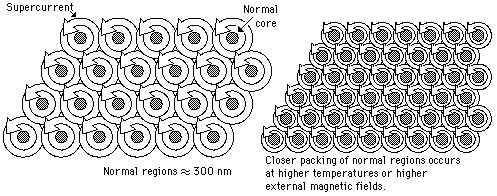
\includegraphics[scale=0.006]{svort}
    \end{center}
    \end{figure}


\end{frame}



\begin{frame}
    \frametitle{Second-order Phase Transitions}
    Second order phase transitions occur when a new state of
reduced symmetry
develops continuously from the
disordered (high temperature) phase. 

\\~\\
The ordered phase has a
lower symmetry
than the Hamiltonian -- the
phenomenon of
spontaneously broken symmetry.
\\~\\
i.e.\ the difference between Type I and Type II superconductors.

\end{frame}

\begin{frame}[<+->]
    \frametitle{Superfluids}

    Interestingly, superfluids have these same vortices, just under different
    conditions.

    \begin{figure}
    \begin{center}
        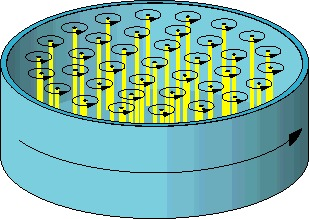
\includegraphics[scale=0.006]{superfluidvort}
    \end{center}
    \end{figure}

\end{frame}


\begin{frame}
    \frametitle{Superfluid Vortices}

    These quantized vortices align with the axis of rotation and form a
    triangular lattice.
    \\~\\

    The resulting course-grain flow closely approximates the analogous
    situation in classical fluid even though quantum mechanics imposes
    stringent constraints on vorticity.

\end{frame}


\begin{frame}
    \frametitle{Aside}

    The zero point energy of liquid helium is less if its atoms are less 
    confined by their neighbors. Hence in liquid helium, its ground 
    state energy can decrease by a naturally-occurring increase in 
    its average interatomic distance.
    \\~\\
    The zero-point energy is the lowest possible energy that a 
    quantum mechanical physical system may have.
    \\~\\
    Because of the very weak interatomic forces in helium, this element 
    would remain a liquid at atmospheric pressure all the way from its 
    liquefaction point down to absolute zero. Liquid helium solidifies 
    only under very low temperatures and great pressures.
\end{frame}





\begin{frame}
    \frametitle{Questions}

    Questions?


\end{frame}







\end{document}
